%
%   This program is free software: you can redistribute it and/or modify
%   it under the terms of the GNU General Public License as published by
%   the Free Software Foundation, either version 3 of the License, or
%   (at your option) any later version.
%
%   This program is distributed in the hope that it will be useful,
%   but WITHOUT ANY WARRANTY; without even the implied warranty of
%   MERCHANTABILITY or FITNESS FOR A PARTICULAR PURPOSE.  See the
%   GNU General Public License for more details.
%
%   You should have received a copy of the GNU General Public License
%   along with this program.  If not, see <http://www.gnu.org/licenses/>.
%

% Version: $Revision: 8032 $

The plugin architecture of the Knowledge Flow allows you to add new steps
and perspectives easily. Plugins for the Knowledge Flow are managed by the
/textit{PluginManager} class and can easily be deployed by creating a 
WEKA package (see Chapter 19) that includes a \textit{PluginManager.props}
file that lists the components to add.

The source code for all the examples described in the following
sections are available in the \textit{newKnowledgeFlowStepExamples}
package that can be installed via the package manager.

\subsection{Creating a simple batch processing Step}
Steps are the building blocks of Knowledge Flow processes. The new
Knowledge Flow implementation has a fresh API and a collection of
helper classes that makes creating a new Step fairly simple.

The need-to-know API elements for new Steps are:

\begin{itemize}
\item \texttt{weka.knowledgeflow.steps.Step} - the main interface for Step implementations
\item \texttt{weka.knowledgeflow.steps.BaseStepExtender} - a minimal subset of the
  \texttt{Step} interface's methods that a new Step would need to
  implement in order to function as a start point and/or processing
  step in the Knowledge Flow.
\item \texttt{weka.knowledgeflow.steps.BaseStep} - a handy base class
  for new Steps to extend. Provides functions for automatically setting up 
  the Step's name and ``about'' info, resolving environment variables
  and gaining access to the Step's \texttt{StepManager} class. This
  class implements \texttt{Step} and \texttt{BaseStepExtender}.
\item \texttt{weka.knowledgeflow.StepManager} - an implementation of
  \textit{StepManager} is provided to every Step by the Knowledge Flow
  environment. \texttt{StepManager} has lots of utility functions that
  allow a Step to find out information about things such as its
  incoming connections, outgoing connections, and execution
  environment. It also provides methods to handle the output of data
  and for informing the Knowledge Flow environment of the Step's
  status.
\item \texttt{weka.knowledgelfow.steps.KFStep} - a class annotation
  that Step implementations can use for specifying their name,
  category, tool tip and icon path.
\end{itemize}

Lets take a look at a simple Step that can accept batch datasets and
compute summary statistics for a user-specified attribute.

\subsection*{Implementation}

Our new \texttt{StatsCalculator} step extends \texttt{BaseStep}. As \texttt{BaseStep}
is abstract, the methods that we must implement are shown in the skeleton class below:

\begin{verbatim}
public class StatsCalculator extends BaseStep {

  @Override
  public void stepInit() throws WekaException {
    // TODO
  }

  @Override
  public List<String> getIncomingConnectionTypes() {
    // TODO
    return null;
  }

  @Override
  public List<String> getOutgoingConnectionTypes() {
    // TODO
    return null;
  }
}
\end{verbatim}

The \textit{stepInit()} function is called on all steps before the
knowledge flow starts executing a flow. It allows a step to reset its
state and check the validity of any user-specified configuration. At
this point the Step is guaranteed to have access to a
\texttt{StepManager}.

The \textit{getIncomingConnectionTypes()} method allows a Step to
specify which incoming connection types it can accept. This should
take into account the current configuration of the step and any
existing connections in (or out) of the step (e.g. a step might only
allow one incoming \textit{trainingSet} connection, so if one is
already present then the list of connection types returned by this
method should not include \textit{trainingSet}).

Similarly, the \textit{getOutgoingConnectionTypes()} method allows the
Step to specify which outgoing connection types can be made from
it. Again, this should take into account the current state of the step
and (possibly) the incoming connections.

Lets take a look at implementing these methods in
\verb=StatsCalculator=.:

\begin{verbatim}
public class StatsCalculator extends BaseStep {

  protected String m_attName = "petallength";

  @Override
  public void stepInit() throws WekaException {
    if (m_attName == null || m_attName.length() == 0) {
      throw new WekaException("You must specify an attribute to compute "
        + "stats for!");
    }
  }

  @Override
  public List<String> getIncomingConnectionTypes() {
    return Arrays.asList(StepManager.CON_DATASET, StepManager.CON_TRAININGSET,
      StepManager.CON_TESTSET);
  }

  @Override
  public List<String> getOutgoingConnectionTypes() {
    List<String> outgoing = new ArrayList<String>();
    if (getStepManager().numIncomingConnections() > 0) {
      outgoing.add(StepManager.CON_TEXT);
    }
    if (getStepManager().numIncomingConnectionsOfType(
      StepManager.CON_DATASET) > 0) {
      outgoing.add(StepManager.CON_DATASET);
    }
    if (getStepManager().numIncomingConnectionsOfType(
      StepManager.CON_TRAININGSET) > 0) {
      outgoing.add(StepManager.CON_TRAININGSET);
    }
    if (getStepManager().numIncomingConnectionsOfType(
      StepManager.CON_TESTSET) > 0) {
      outgoing.add(StepManager.CON_TESTSET);
    }
    return outgoing;
  }
}
\end{verbatim}

The code specifies that the step can accept any number of incoming
\texttt{dataset}, \texttt{trainingSet} or \texttt{testSet}
connections. There are a whole lot of constants defined in
\texttt{StepManager} for connection types and auxilliary data. The
\textit{getOutgoingConnectionTypes()} method specifies that the step
will only produce a \texttt{text} connection/output if it has at least
one incoming connection. The \texttt{text} output will contain our
computed attribute summary statistics. Furthermore, the step also
passes through any instances that it receives, so it will only produce
a particular dataset type (\texttt{dataSet}, \texttt{trainingSet} or
\texttt{testSet}) if it has a corresponding inpcoming connection of
that type.

At this point there is some important functionality missing - namely a
method to do some actual processing when data is received by the
step. In fact, there are two methods related to this in
\texttt{BaseStep} that have no-opp implementations. One or both should
be overridden by a \verb=Step= implementation in order to do some
processing. the \textit{start()} method should be overriden if the
step can act as a starting point in a flow (i.e. a step that,
typically, loads, sources or generates data of some sort). Any step
that doesn't have any incoming connections is considered as a
potential start point by the Knowledge Flow environment and has its
\textit{start()} method invoked. The \textit{processIncoming()} method
should be overridden by steps that can accept incoming connections
(and the data that they typically carry).

Lets add a \textit{processIncoming()} method to the \verb=StatsCalculator=.

\begin{verbatim}
  public void setAttName(String attName) { m_attName = attName; }

  public String getAttName() { return m_attName; }

  @Override
  public void processIncoming(Data data) throws WekaException {
    getStepManager().processing();
    Instances insts = data.getPrimaryPayload();
    Attribute att = insts.attribute(getAttName());
    if (att == null) {
      throw new WekaException("Incoming data does not " + "contain attribute '"
        + getAttName() + "'");
    }
    AttributeStats stats = insts.attributeStats(att.index());
    Data textOut = new Data(StepManager.CON_TEXT, stats.toString());
    textOut.setPayloadElement(StepManager.CON_AUX_DATA_TEXT_TITLE,
      "Stats for: " + getAttName());
    getStepManager().outputData(textOut); // output the textual stats
    getStepManager().outputData(data); // pass the original dataset on
    getStepManager().finished();
  }
\end{verbatim}

In the code above, we've added accessor and mutator methods for our
single user-supplied parameter - i.e. the name of the attribute to
compute stats for. Then we've overridden the no-opp implementation of
the \textit{processIncoming()} method from \verb=BaseStep=. This
method is passed a \verb=Data= object, which is the data structure
used by the Knowledge Flow environment for transferring all types of
data between steps. The code first tells the Knowledge Flow
environment that it is actively processing by calling the
\textit{processing()} method on the step's \verb=StepManager=. It then
retrieves the \verb=Instances= dataset via the
\textit{getPrimaryPayload()} method of the \verb=Data= object. The
stats are then computed and a new \verb=Data= object is created to
hold the results. In this case the results are textual, so the data's
associated connection type is \verb=StepManager.CON_TEXT=. The two
argument constructor for \verb=Data= takes the connection type and the
associated primary payload data (i.e. the textual stats in this
case). Additional data can be attached to a \verb=Data= object by
storing it in a ``payload'' map. In this case we have a textual title
for our stats result that includes the name of the attribute. Finally,
the new data object, and the original dataset, is output by calling
the \textit{outputData()} method on the \verb=StepManager=, and the
environment is informed that our step has finished processing.

The last thing we can add to this step is the \verb=KFStep= class
annotation. This provides some information about the step, including
where it should appear in the folders of the design palette in the
GUI Knowledge Flow.

\begin{verbatim}
@KFStep(name = "StatsCalculator", category = "Examples",
  toolTipText = "Compute summary stats for an attribute",
  iconPath = KFGUIConsts.BASE_ICON_PATH + "DiamondPlain.gif")
public class StatsCalculator extends BaseStep {

...
\end{verbatim}


\begin{center}
  \includegraphics[width=12cm]{images/knowledgeflow/statsCalc.eps}
\end{center}

The screenshot above shows the step, the results after execution on
the iris data and the GUI configuration dialog for the step. A simple,
GUI configuration dialog is provided dynamically by the Knowledge Flow
environment, but you have the option of overriding this to a greater
or lesser extent in order to provide a customized configuration
dialog.

\subsection{Creating a simple streaming Step}
\verb=StepManager= defines a number of constant strings that identify
various types of connections and data. Most data/connections in the
Knowledge Flow are batch ones - e.g. \textit{dataSet},
\textit{trainingSet}, \textit{testSet} and \textit{batchClassifier}
(to name a few). When the Knowledge Flow's execution environment
invokes \textit{processIncoming()} on a target step, it does so in a
separate thread for batch connections. Thus, each step automatically
does its processing within a separate thread. There are several types
of incremental connections/data defined in \verb=StepManager= as well:
\textit{instance}, \textit{incrementalClassifier} and \textit{chart}
are all examples. Furthermore, for your own purposes it is possible to
create your own connection/data types (as they are just defined with a
string identifier) and mark them as ``incremental''. This can be done
by setting payload flag
(\verb=StepManager.CON_AUX_DATA_IS_INCREMENTAL= to \verb=true=) when
configuring a \verb=Data= object. Incremental connections/data do not
get executed in a new thread because it is assumed that processing
individual pieces of incremental data does not require much effort,
and the overhead in creating/invoking processing in a new thread could
outweigh this.

Now lets take a look at a \verb=Step= that does some simple processing
in a streaming fashion. Our new step, \verb=RoundRobin=, simply
accepts a single streaming ``instance'' connection as input and
distributes individual instances in a round-robin fashion to the
connected steps immediately downstream from it.

\subsection*{Implementation}

\begin{verbatim}
@KFStep(name = "RoundRobin", category = "Examples",
  toolTipText = "Round robin instances to outputs",
  iconPath = KFGUIConsts.BASE_ICON_PATH + "DiamondPlain.gif")
public class RoundRobin extends BaseStep {
  protected int m_counter;
  protected int m_numConnected;

  @Override
  public void stepInit() throws WekaException {
    m_counter = 0;
    m_numConnected = getStepManager().numOutgoingConnections();
  }

  @Override
  public List<String> getIncomingConnectionTypes() {
    List<String> result = new ArrayList<String>();
    if (getStepManager().numIncomingConnections() == 0) {
      result.add(StepManager.CON_INSTANCE);
    }
    return result;
  }
  @Override
  public List<String> getOutgoingConnectionTypes() {
    List<String> result = new ArrayList<String>();
    if (getStepManager().numIncomingConnections() == 1) {
      result.add(StepManager.CON_INSTANCE);
    }
    return result;
  }

  @Override
  public void processIncoming(Data data) throws WekaException {
    if (isStopRequested()) {
      getStepManager().interrupted();
      return;
    }
    if (getStepManager().numOutgoingConnections() > 0) {
      getStepManager().throughputUpdateStart();
      if (!getStepManager().isStreamFinished(data)) {
        List<StepManager> outgoing =
          getStepManager().getOutgoingConnectedStepsOfConnectionType(
            StepManager.CON_INSTANCE);
        int target = m_counter++ % m_numConnected;
        String targetStepName = outgoing.get(target).getName();
        getStepManager().outputData(StepManager.CON_INSTANCE, targetStepName,
          data);
        getStepManager().throughputUpdateEnd();
      } else {
        // step manager notifies all downstream steps of stream end
        getStepManager().throughputFinished(data);
      }
    }
  }
}
\end{verbatim}
\newpage

This example step demonstrates a several different things over the one
in the previous section. Firstly the
\textit{getIncomingConnectionTypes()} and
\textit{getOutgoingConnectionTypes()} methods demonstrate some
constraints based on the current state of incoming and outgoing
connections. In the former method a constraint of a single incoming
\verb=instance= connection is enforced; in the later method any number
of outgoing \verb=instance= connections are allowed as long as there
is an incoming connection present. It also demonstrates checking to
see whether a request has been made to stop processing in the
\textit{processIncoming()} method. We ommitted this from the previous
example for brevity, but all steps should check periodically to see if
a stop has been requested. If so, then they should indicate to the
environment as soon as possible that they have been interrupted by
calling \textit{StepManager.interrupted()}. This method will ensure
that an interruped message appears in the status area of the GUI
Knowledge Flow.

The code also demonstrates several features of incremental processing
in the \textit{processIncoming()} method. To get throughput statistics
displayed in the status area of the GUI Knowledge Flow interface the
methods \textit{StepManager.throughputUpdateStart()} and
\textit{StepManager.throughputUpdateEnd()} are used to indicate the
start and end of processing for the incoming \verb=Data= object
respectively. A utility method \textit{StepManager.isStreamFinished()}
can be called to see if the end of the stream has been reached. This
method takes the current \verb=Data= object (as a flag is set in the
payload map of the \verb=Data= object to indicate the end of the
stream). By convention, the primary payload of a \verb=Data= object
that is marked as end-of-stream is empty/null. However, auxilliary
data could be present, depending on what processing has been done
(e.g. a final classifier object if training a classifier
incrementally). If the end of stream has been reached, then a step
should call \textit{StepManager.throughputFinished()} with a final
\verb=Data= object as an argument - this tells the environment that
processing is finished for the step and ensures that downstream steps
are informed of the end-of-stream along with any final auxilliary data
in the final \verb=Data= object.

In the previous example, we had simply output data to all downstream
steps with the appropriate connection type by calling
\textit{StepManager.outputData()} with a single \verb=Data= object as
an argument. The environment routes this data to appropriate connected
steps because the \verb=Data= object is constructed with a connection
type that it is associated with. In our round robin example, we
further constrain the destination of the data by calling a version of
\textit{StepManager.outputData()} that takes a step name as an additional
argument.

\subsection{Features of StepManager}

Aside from methods to query the state of incoming and outgoing connections
from a step, and support for outputing data, the \verb=StepManager= also
has a number of other useful facilities. It provides methods for writing
to the status and log in the KnowledgeFlow. Messages can be logged at
various logging levels, where the user can configure up to which level
they are interested in seeing in the log. The following status and logging
methods can be used by steps during execution:

\begin{tight_itemize}
  \item \verb=statusMessage()= - write to the status area
    \item \verb=logLow()=
    \item \verb=logBasic()=
    \item \verb=logDetailed()=
    \item \verb=logDebug()=
    \item \verb=logWarning()= - always gets to the log, regardless of user-specified logging level
    \item \verb=logError()= - always gets to the log; can supply an optional \verb=Throwable= cause
\end{tight_itemize}

\verb=StepManager= also provides access to the
\verb=ExecutionEnvornment=. The \verb=ExecutionEnvironment= can be
used to find out whether the system is running headless, get the
values of environment variables and to launch separate processing
``tasks'' on the executor service. In most cases, the processing done
by a step will not require launching additional tasks/threads as
\textit{processIncoming()} is called in a separate thread (when batch
processing) by the Knowledge Flow environment. In some cases, it might
be beneficial to make use of additional threads. The
\textit{BoundaryPlotter} step is an example that makes use of this
facility - it computes each row of a plotted graphic using a separate
task/thread. Steps wanting to use the executor service directly can
call \textit{StepManager.getExecutionEnvironment().submitTask()} and
supply a concrete sublcass of \verb=StepTask= to do the
processing. The step can work with either the
\verb=Future<ExectutionResult>= returned by \textit{submitTask()} or,
alternatively, supply a \verb=StepTaskCallback= when constructing a
\verb=StepTask= for asynchronous notification.

\subsection{PairedDataHelper}

A common processing pattern in machine learning is to deal with paired
datasets - i.e. typically train/test pairs. In the multi-threaded
environment of the Knowledge Flow, where usually each \verb=Data=
object is passed to a target step in a separate thread of execution,
it is likely that training and test sets may arrive at the target step
out of order. Furthermore, in the case of multiple pairs
(e.g. cross-validation folds) they might not arrive in the order that
the folds are created. Handling this scenario within a step can be
tedious, so a helper class is available for use by step
implementations needing to deal with paired datasets -
\verb=PairedDataHelper=.

The \verb=PairedDataHelper= has the concept of a primary and secondary
connection/data type, where the secondary connection/data for a given
set number typically needs to be processed using a result generated
from the corresponding primary connection/data. This class takes care
of ensuring that the secondary connection/data is only processed once
the primary has completed. Users of this helper need to provide an
implementation of the \verb=PairedProcessor= inner interface, where
the \textit{processPrimary()} method will be called to process the
primary data/connection (and return a result), and
\textit{processSecondary()} called to deal with the secondary
connection/data. The result of execution on a particular primary data
set number can be retrieved by calling the
\textit{getIndexedPrimaryResult()} method, passing in the set number
of the primary result to retrieve.

The \verb=PairedDataHelper= class also provides an arbitrary storage
mechanism for additional results beyond the primary type of result. It
also takes care of invoking \textit{processing()} and
\textit{finished()} on the client step's \verb=StepManager=.

Below is a code skeleton (taken from the javadoc for
\verb=PairedDataHelper=) that shows the basic usage of this helper
class.

\begin{verbatim}
public class MyFunkyStep extends BaseStep
  implements PairedDataHelper.PairedProcessor<MyFunkyMainResult> {
   ...
   protected PairedDataHelper<MyFunkyMainResult> m_helper;
   ...
   public void stepInit() {
     m_helper = new PairedDataHelper<MyFunkyMainResult>(this, this,
     StepManager.[CON_WHATEVER_YOUR_PRIMARY_CONNECTION_IS],
     StepManager.[CON_WHATEVER_YOUR_SECONDARY_CONNECTION_IS]);

      ...
    }

    public void processIncoming(Data data) throws WekaException {
      // delegate to our helper to handle primary/secondary synchronization
      // issues
      m_helper.process(data);
    }

    public MyFunkyMainResult processPrimary(Integer setNum, Integer maxSetNun,
      Data data, PairedDataHelper<MyFunkyMainResult> helper) throws WekaException {
      SomeDataTypeToProcess someData = data.getPrimaryPayload();
 
      MyFunkyMainResult processor = new MyFunkyMainResult();
      // do some processing using MyFunkyMainResult and SomeDataToProcess
      ...
      // output some data to downstream steps if necessary
      ...
   
      return processor;
    }
   
    public void processSecondary(Integer setNum, Integer maxSetNum, Data data,
      PairedDataHelper<MyFunkyMainResult> helper) throws WekaException {
      SomeDataTypeToProcess someData = data.getPrimaryPayload();
   
      // get the MyFunkyMainResult for this set number
      MyFunkyMainResult result = helper.getIndexedPrimaryResult(setNum);
   
      // do some stuff with the result and the secondary data
           ...
      // output some data to downstream steps if necessary
    }
}

\end{verbatim}

The \textit{newKnowledgeFlowStepExamples} package includes an example
called \verb=ExampleClassifier= that demonstrates the use of
\verb=PairedDataHelper= to train and evaluate a classifier on
train/test splits.
